\documentclass{article}
\usepackage{amsmath}
\usepackage{url}
\usepackage{graphicx}
%	\addtolength{\oddsidemargin}{-.5in}
%	\addtolength{\evensidemargin}{-.5in}
%	\addtolength{\textwidth}{0.75in}
%	\addtolength{\topmargin}{-1in}
%	\addtolength{\textheight}{1.75in}
\title{Final Year Project Interim Report\\ Content-based Prediction of Web 2.0 Page Updates}
\author{U096883L Shawn Tan}
\date{}
\begin{document}
\maketitle
\section{Introduction}
With the increasing number of Web 2.0 sites, sites with forums, or similar thread-based discussion features are extremely common. Data found on discussions like these provide useful feedback for content providers. As more users are involved with the content-generation process of these sites, maintaining an updated database of crawled content becomes increasingly difficult.


\begin{table}\label{table:web20}
	\begin{center}
	{\footnotesize
	\begin{tabular}{|l|c|c|c|c|c|c|c|c|c|c|}
		\hline
			\input{web20}
		\hline
	\end{tabular}
	}
\end{center}
\caption{Features of popular Web 2.0 sites}
\end{table}

Looking at Table \ref{table:web20}, we find that many of the popular Web 2.0 sites have a comment feature. This suggests that content on the web is increasingly being created by users rather than content providers. While mining structured, curated content from sites like Amazon, for data like prices may be effective, data that can be obtained from user-generated content are of a different nature. One may be able to infer public sentiment about a given product, for example.

Web crawlers can be used to crawl sites for user comments and threads for postprocessing later. Web crawlers which maintain the `freshness' of a database of crawled content are known as incremental crawlers. Two tradeoffs these crawlers face cited by Yang et. al. 2009 \cite{Yang2009} are \emph{completeness} and \emph{timeliness}. \emph{Completeness} refers to the extent which the crawler fetches all the pages, without missing any pages. \emph{Timeliness} refers to the efficiency with which the crawler discovers and downloads newly created content.

Let us define all such thread-based discussion styled sites as forums. Ideally, an incremental crawler of such user-generated content should be able to maintain a fresh and complete database of content of the forum that it is monitoring. A naive way to approach this would be to aggressively download these pages at a frequent rate. This, however, would (1) incur excessive costs when downloading un-updated pages, and (2) raise the possibility of the web master blocking the requester's IP address.


Thus, we need a strategy of revisiting pages that will reduce the cost of downloading unchanged pages, while at the same time downloading them as soon as possible after it's update.

\section{Related work}
In order to devise such a strategy, we need to predict how often any user may update the a page. Some work has been done to try to predict how often page content is updated by the page owner.

Many such works have used the Poisson distribution to model page updates. Coffman et. al. \cite{Coffman1997} analysed the theoretical aspects of doing this, while Cho and Garcia-Molina trace the change history of 720,000 web pages collected over 4 months, and compared the result against what the Poisson process model predicts \cite{Cho1999}, and then proposed different revisiting or refresh policies \cite{Cho2003,Garcia-molina2003} that attempt to maintain the `freshness' of the database. The Poisson distribution were also used in Tan et. al. \cite{Tan2007} and Wolf et. al. \cite{Wolf2002}. %elaborate!!!!
However, the Poisson distribution is memoryless, and in experimental results due to Brewington and Cybenko \cite{Brian2000}, the behaviour of site updates are not.

Yang et. al. \cite{Yang2009}, attempted to resolve this by using the list structure of forum sites to infer a sitemap. With this, they reconstruct the full thread, and then use a linear-regression model to predict when the next update to the thread will arrive. %elaborate!!!

These methods of estimating page updates either rely on previously gathered information about the page updates through repeated polling of the page, or through timestamps gathered from the individual posts. They have two shortfalls:

\begin{description}
	\item[Lack/Improperly formatted Timestamp Information] While most comment threads or forum sites tend to have timestamps, they often try to optimise readability. For example, timestamps of comments that were posted 8 months ago may be displayed as ``more than 4 months ago''.
	\item[Requires previous time series data]
		If the individual threads are treated independently of each other, a new thread (1 or 2 posts) would not have sufficient data to fit a Poisson model. Yang et. al. \cite{Yang2009} accounts for this by factoring into their regression model other threads with a similar recent history
\end{description}
The lack of these pieces of information may result in a poorer estimate, or no estimate at all. We argue, that the content within the posts of the thread should be important in predicting the thread updates. While there is little existing work using content to predict page updates, we will review some existing work related to analysing thread-based pages which we think will aid us in our efforts to do content-based prediction.

Kleinberg \cite{Kleinberg2002} used Hidden Markov Models to predict ``bursts" in message arrival times. In his running example, he used email messages, and used time between messages to estimate the states that produced the sequence. While the model may be able to predict what the state is for the next time interval, it does so using the history of message arrival times, and does not take into account the content within the messages themselves.

One work related to evaluating content on threads relates to finding out linkages between forum posts using lexical chaining. They proposed a method to link posts using the tokens in the posts called $Chainer_{SV}$. While they do analyse the content of the individual posts, the paper does not make any prediction with regards to newer posts.



\section{Possible Approaches}

\subsection{Hidden Markov Models}
One possible way of forecasting the next forum post would be to model each thread as having a state that describes its activity level, ``Idle" or ``Active" for example. At any time $t$, it transitions to other states or stays at its current state with a given probability $T(s,s')$.

The objective, is to infer the observations made to each state with regards to content.


\subsection{Lexical Chaining}
Another way to leverage the content in the thread might be to look at the post linkage structure. Lexical chaining gives a numerical relationship between theach post in the thread. Analysing the time between these posts and the lexical chains, we may be able to predict, given the posts in the thread, when the next post may arrive.

\section{Preliminary work}
\begin{figure}
	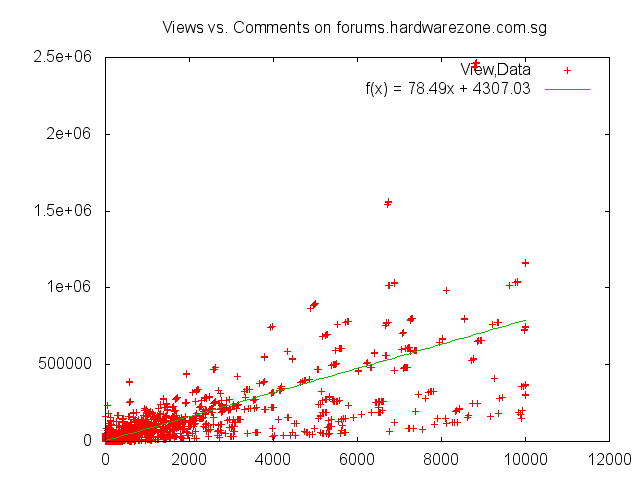
\includegraphics[scale=0.5]{view-comment.png}
	\caption{Linear fit of Views vs Comments from forum.hardwarezone.com.sg}
\end{figure}

\bibliographystyle{acm}
\bibliography{report}
\end{document}
